\section{离散信号}

本节介绍离散信号,并给出2种基本的离散信号。

本节要点:
\begin{itemize}
    \item 掌握离散信号的概念;
    \item 熟悉2个基本离散信号。
\end{itemize}

%============================================================
\subsection{离散信号的概念}

\begin{definition}[离散信号]
当时间变量取离散值$t=t_n,n=0,\pm 0,\pm 2,\cdots $时,我们称信号为{\bf 离散信号}(discrete-time signal),记为$x\left[ n \right] $,其中$n$表示$t_n$,即第$n$个时间采样点。
一般我们通过对连续信号的周期性采样获得离散信号,即:
\begin{align*}
&n=\frac{t}{T} \\
&x\left[ n \right] =\left. x\left( t \right) \right|_{t=nT}=x\left( nT \right)
\end{align*}
其中,$T$为采样周期,单位s。
\end{definition}

虽然不硬性规定$t_n$之间的间隔,但一般我们还是等间隔处理,即“周期性”采样。

%============================================================
\subsection{单位阶跃和单位冲激}

\begin{figure}[h]
\centering
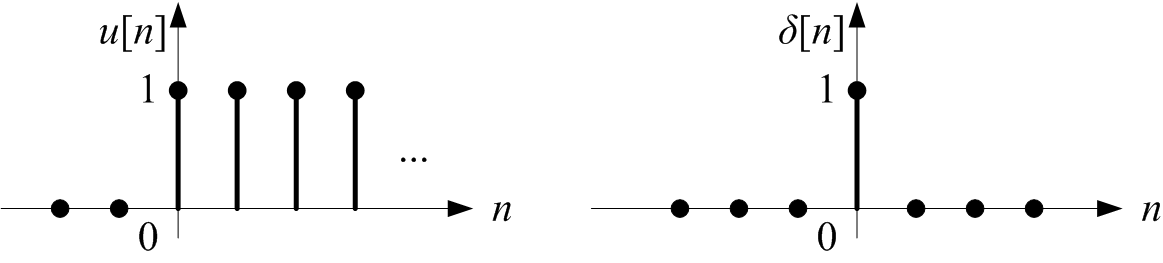
\includegraphics[height=2cm]{1.3.2-1.png}
\end{figure}
\[
u\left[ n \right] =\begin{cases}
	1 \quad n=0,1,2,\cdots\\
	0 \quad n=-1,-2,\cdots\\
\end{cases} \quad \delta \left[ n \right] =\begin{cases}
	1 \quad n=0\\
	0 \quad n=\pm 1,\pm 2,\cdots\\
\end{cases}
\]




